\documentclass{article}

\usepackage{arxiv}
\usepackage[T1]{fontenc}
\usepackage[utf8]{inputenc}
\usepackage[english]{babel}
\usepackage{microtype}

\usepackage{amsmath}
\usepackage{amssymb}
\usepackage{amsthm}
\usepackage{mathtools}
\usepackage{float}
\usepackage{booktabs}
\usepackage{caption}
\usepackage{subcaption}
\usepackage{tikz}
\usepackage[autostyle=true]{csquotes}
\usepackage[hidelinks]{hyperref}

\theoremstyle{plain}
\newtheorem{theorem}{Theorem}
\newtheorem{lemma}[theorem]{Lemma}
\newtheorem{corollary}[theorem]{Corollary}
\theoremstyle{definition}
\newtheorem{definition}[theorem]{Definition}
\newtheorem{remark}[theorem]{Remark}

\newcommand{\R}{\mathbb{R}}
\newcommand{\Ha}{\mathbb{H}}
\newcommand{\vect}[1]{\boldsymbol{#1}}
\newcommand{\tr}{\operatorname{tr}}
\newcommand{\lean}[1]{\texttt{#1}}

%----------------------------------------------------------------------
% Coordinate frame figures
%
% \coordframe{x vector}{y vector}{z vector}{title}{angle x}{angle y}{angle z}{title y position}
%
% The three vectors are the screen directions of the frame's own x, y, z axes.
% Each arc is drawn in the frame's own coordinates from the first to the second
% axis of the rotation plane (x: y -> z, y: z -> x, z: x -> y). This is the
% positive sense of R_x, R_y, R_z in every frame, so right-handed frames show the
% right-hand rule and left-handed frames the left-hand rule automatically.
%----------------------------------------------------------------------
\definecolor{axiscol}{RGB}{31,78,140}
\definecolor{rotcol}{RGB}{200,90,20}
\tikzset{
  axis/.style={-latex, line width=1.1pt, axiscol},
  rot/.style={-latex, line width=0.9pt, rotcol},
  angle/.style={rotcol, inner sep=1pt},
}
\newcommand{\coordframe}[8]{%
  \begin{scope}[scale=1.5, x={#1}, y={#2}, z={#3}]
    \draw[axis] (0,0,0) -- (1.8,0,0) node[pos=1.07, black] {$x$};
    \draw[axis] (0,0,0) -- (0,1.8,0) node[pos=1.07, black] {$y$};
    \draw[axis] (0,0,0) -- (0,0,1.8) node[pos=1.07, black] {$z$};
    \draw[rot] plot[domain=35:315, smooth, samples=40, variable=\t]
      ({1.25}, {0.32*cos(\t)}, {0.32*sin(\t)});
    \draw[rot] plot[domain=35:315, smooth, samples=40, variable=\t]
      ({0.32*sin(\t)}, {1.25}, {0.32*cos(\t)});
    \draw[rot] plot[domain=35:315, smooth, samples=40, variable=\t]
      ({0.32*cos(\t)}, {0.32*sin(\t)}, {1.25});
    \node[angle] at ({1.25}, {0.6*cos(215)}, {0.6*sin(215)}) {#5};
    \node[angle] at ({0.6*sin(215)}, {1.25}, {0.6*cos(215)}) {#6};
    \node[angle] at ({0.6*cos(215)}, {0.6*sin(215)}, {1.25}) {#7};
  \end{scope}
  \node[font=\bfseries\small] at (1.4,#8) {#4};
}
\title{Converting Poses between Right-Handed and Left-Handed Coordinate Systems: Quaternions, Euler Angles and Rotation Matrices}
\author{Felix Weichselgartner}
\date{}
\renewcommand{\shorttitle}{Converting Poses between Right-Handed and Left-Handed Systems}

\begin{document}
\maketitle

\begin{abstract}
Mathematics and robotics almost exclusively use right-handed coordinate systems, whereas
game engines such as Unity3D often use left-handed ones. Whenever both worlds are connected,
positions and rotations have to be transferred from one system to the other. The required
sign rules are widely used in practice, but they are usually given case by case, without
derivation and sometimes contradicting each other. This tutorial collects the conversion in one
place. If the coordinates of the two systems differ by an orthogonal matrix $\vect P$ with
$\det \vect P = -1$, the position is transformed with $\vect P$, the rotation matrix with
$\vect P(\cdot)\vect P^T$, and the vector part of the quaternion with $-\vect P$ while the scalar
part is kept. This follows from the transformation law of axial vectors. Two cases are worked out
in full: a mirrored $z$ axis, and swapped $y$ and $z$ axes as in Unity3D. Common pitfalls are
listed. All statements about both cases are proved formally in the proof assistant Lean~4 with
Mathlib.
\end{abstract}

\keywords{quaternions \and Euler angles \and rotation matrix \and handedness \and
coordinate transformation \and formal verification}

%======================================================================
\section{Introduction}\label{sec:intro}

Figure~\ref{fig:handedness} shows a right-handed and a left-handed coordinate system. Both are
chiral: no rotation turns a right-handed system into a left-handed one, a reflection is always
required. The axes of a right-handed system follow the right-hand rule (thumb $x$, index finger
$y$, middle finger $z$), and a positive rotation turns counterclockwise when viewed from the tip
of the axis (right-fist rule). For a left-handed system the left-hand rule and the left-fist rule
apply, so positive rotations turn clockwise.

\begin{figure}[H]
  \centering
  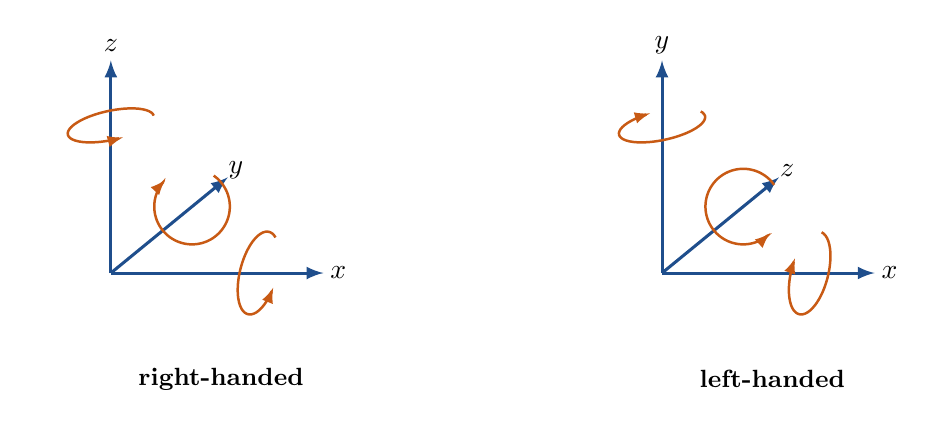
\begin{tikzpicture}
    \coordframe{(1cm,0cm)}{(0.55cm,0.45cm)}{(0cm,1cm)}{right-handed}{}{}{}{-1.35}
    \begin{scope}[xshift=7cm]
      \coordframe{(1cm,0cm)}{(0cm,1cm)}{(0.55cm,0.45cm)}{left-handed}{}{}{}{-1.35}
    \end{scope}
  \end{tikzpicture}
  \caption{Right-handed and left-handed coordinate system. The arrows show the positive
  direction of rotation about each axis.}
  \label{fig:handedness}
\end{figure}

Anyone who wants to display a pose (position and rotation) from a right-handed system, for
example from a camera calibration or a robot controller, in a game engine with a left-handed
system has to convert both parts. For the position this is obvious, for the rotation it is not:
merely reordering the quaternion components generally yields a wrong orientation.

The underlying mathematics is not new. The vector part of a rotation quaternion behaves like an
axial vector, and axial vectors pick up the factor $\det \vect P$ under an improper change of basis.
What is missing, to our knowledge, is a source that states the conversion for a general change of
handedness, proves it, and covers positions, rotation matrices, Euler angles and quaternions
consistently (Section~\ref{sec:related}). This paper is meant as such a reference for practitioners,
for example when connecting robotics or computer vision software to a game engine.

Contributions of this paper:
\begin{itemize}
  \item a unified statement of the conversion rule for positions, rotation matrices and
        quaternions for any change of handedness (Theorem~\ref{thm:main}), with proof,
  \item a complete calculation of two practically relevant cases
        (Sections~\ref{sec:ex1} and~\ref{sec:ex2}), including the proof that the conversion via
        rotation matrices and the direct conversion from Euler angles agree in all four
        quaternion components,
  \item a list of common pitfalls (Section~\ref{sec:pitfalls}),
  \item a formal verification of all statements about both cases in Lean~4
        (Section~\ref{sec:lean}).
\end{itemize}

%======================================================================
\section{Related work}\label{sec:related}

\paragraph{Practice.} Sign rules for converting quaternions between right-handed and left-handed
systems circulate in forum answers, blog posts and source code, for example in the Unity
community \cite{unityforum}, in tutorials \cite{codeproject} and in libraries such as Unity's
ROS-TCP-Connector, which converts between the ROS frame (forward, left, up) and the Unity frame
(right, up, forward) \cite{rosgeometry}. These sources give a rule for one specific pair of
systems, usually without derivation. Since they assume different axis mappings, their rules
differ, which makes it hard to tell which rule applies to a new pair of systems.

\paragraph{Attitude representations.} The standard references on rotation representations treat
proper rotations only. Diebel \cite{diebel2006} explicitly restricts the analysis to proper
rotations because improper rotations are not rigid-body transformations. Shuster
\cite{shuster1993} surveys attitude representations. Sol\`a \cite{sola2017} and Sommer
et al.\ \cite{sommer2018} discuss the conventions of quaternions in detail: component order,
active vs.\ passive use, and the handedness of the quaternion \emph{algebra} (Hamilton's
$ij = k$ vs.\ the JPL convention $ij = -k$, whose quaternions are conjugate to each other). This
is a different question from the handedness of the \emph{coordinate system} treated here, and
Sommer et al.\ state explicitly that they do not consider improper rotations.

\paragraph{Reflections and axial vectors.} That the cross product, and with it every axial vector,
picks up the factor $\det \vect P$ under an orthogonal map $\vect P$ is textbook material
\cite{haber}. Reflections expressed with quaternions go back to Coxeter \cite{coxeter1946}.
Theorem~\ref{thm:main} applies this to rotation quaternions.

\paragraph{Formal verification.} Quaternions have been formalized in several proof assistants,
among them HOL Light, Coq, Isabelle/HOL and PVS \cite{itp2024}. We are not aware of a formal proof
of the conversion between right-handed and left-handed systems.

%======================================================================
\section{Preliminaries}\label{sec:prelim}

\subsection{Elementary rotations and conventions}

The rotations about the coordinate axes of a right-handed system by the angles
$\varphi$ ($x$), $\theta$ ($y$) and $\psi$ ($z$) are
\begin{equation}
  \setlength{\arraycolsep}{4pt}
  \vect R_x(\varphi) = \begin{bmatrix} 1 & 0 & 0 \\ 0 & \cos\varphi & -\sin\varphi \\ 0 & \sin\varphi & \cos\varphi \end{bmatrix},\quad
  \vect R_y(\theta) = \begin{bmatrix} \cos\theta & 0 & \sin\theta \\ 0 & 1 & 0 \\ -\sin\theta & 0 & \cos\theta \end{bmatrix},\quad
  \vect R_z(\psi) = \begin{bmatrix} \cos\psi & -\sin\psi & 0 \\ \sin\psi & \cos\psi & 0 \\ 0 & 0 & 1 \end{bmatrix}.
\end{equation}

A general rotation is composed of three elementary rotations. If the first axis is repeated
(e.g.\ ZXZ), the angles are called proper Euler angles, otherwise (e.g.\ YXZ) Tait--Bryan angles.
Independently of this, \emph{intrinsic} rotations about the moving axes multiply from the right
and \emph{extrinsic} rotations about the fixed axes multiply from the left. The matrix used in
this paper,
\begin{equation}\label{eq:yxz}
  \vect R = \vect R_y(\theta)\, \vect R_x(\varphi)\, \vect R_z(\psi),
\end{equation}
therefore describes the intrinsic sequence $y$, $x'$, $z''$ and the extrinsic sequence $z$, $x$, $y$.

The following abbreviations are used:
\begin{equation}
  c_1 = \cos\varphi,\; s_1 = \sin\varphi,\quad
  c_2 = \cos\theta,\; s_2 = \sin\theta,\quad
  c_3 = \cos\psi,\; s_3 = \sin\psi,
\end{equation}
and $c_{kh}$, $s_{kh}$ for the cosine and sine of the half angles.

\subsection{Quaternions}

The quaternions, introduced by Hamilton \cite{hamilton1844} (see \cite{vincequaternions} for a
modern treatment), are
\begin{equation}
  \Ha = \{\, q = q_s + i\,q_x + j\,q_y + k\,q_z \mid q_s, q_x, q_y, q_z \in \R \,\},\qquad
  i^2 = j^2 = k^2 = ijk = -1 .
\end{equation}
We write $q = (q_s, \vect v)$ with scalar part $q_s$ and vector part
$\vect v = (q_x, q_y, q_z)^T$. The conjugate is $q^* = (q_s, -\vect v)$, the norm
$|q|^2 = q_s^2 + q_x^2 + q_y^2 + q_z^2$. The (Hamilton) product is
\begin{equation}
  q_a\, q_b =
  \begin{bmatrix}
    q_{sa} & -q_{xa} & -q_{ya} & -q_{za} \\
    q_{xa} &  q_{sa} & -q_{za} &  q_{ya} \\
    q_{ya} &  q_{za} &  q_{sa} & -q_{xa} \\
    q_{za} & -q_{ya} &  q_{xa} &  q_{sa}
  \end{bmatrix}
  \begin{bmatrix} q_{sb} \\ q_{xb} \\ q_{yb} \\ q_{zb} \end{bmatrix}.
\end{equation}

A unit quaternion $q = \bigl(\cos\tfrac{\alpha}{2},\, \sin\tfrac{\alpha}{2}\,\vect n\bigr)$ with
$|\vect n| = 1$ describes the rotation about the axis $\vect n$ by the angle $\alpha$. A vector
$\vect u$ is rotated by $(0, \vect u') = q\,(0, \vect u)\,q^*$; this representation became the
standard for rotations in computer graphics with \cite{shoemake1985}. The corresponding rotation
matrix is
\begin{equation}\label{eq:Rq}
  \vect R(q) =
  \begin{bmatrix}
    q_s^2 + q_x^2 - q_y^2 - q_z^2 & 2(q_x q_y - q_s q_z) & 2(q_x q_z + q_s q_y) \\
    2(q_x q_y + q_s q_z) & q_s^2 - q_x^2 + q_y^2 - q_z^2 & 2(q_y q_z - q_s q_x) \\
    2(q_x q_z - q_s q_y) & 2(q_y q_z + q_s q_x) & q_s^2 - q_x^2 - q_y^2 + q_z^2
  \end{bmatrix}.
\end{equation}
The map $q \mapsto \vect R(q)$ is multiplicative, $\vect R(q_a q_b) = \vect R(q_a)\,\vect R(q_b)$,
and $q$ and $-q$ describe the same rotation.

\paragraph{Euler angles to quaternion (eul2quat).}
The elementary rotations correspond to
\begin{equation}
  q_x(\varphi) = \cos\tfrac{\varphi}{2} + i \sin\tfrac{\varphi}{2},\quad
  q_y(\theta) = \cos\tfrac{\theta}{2} + j \sin\tfrac{\theta}{2},\quad
  q_z(\psi) = \cos\tfrac{\psi}{2} + k \sin\tfrac{\psi}{2},
\end{equation}
with $\vect R_x(\varphi) = \vect R(q_x(\varphi))$ etc. By multiplicativity, the rotation
\eqref{eq:yxz} has the quaternion $q = q_y(\theta)\, q_x(\varphi)\, q_z(\psi)$.

\paragraph{Rotation matrix to quaternion (rotm2quat).}
For a unit quaternion, \eqref{eq:Rq} gives
\begin{equation}
  \tr \vect R + 1 = 4 q_s^2,\qquad
  R_{32} - R_{23} = 4 q_s q_x,\qquad
  R_{13} - R_{31} = 4 q_s q_y,\qquad
  R_{21} - R_{12} = 4 q_s q_z
\end{equation}
(indices starting at 1). For $q_s > 0$ this yields
\begin{equation}\label{eq:rotm2quat}
  q_s = \frac{\sqrt{\tr \vect R + 1}}{2},\qquad
  q_x = \frac{R_{32} - R_{23}}{4 q_s},\qquad
  q_y = \frac{R_{13} - R_{31}}{4 q_s},\qquad
  q_z = \frac{R_{21} - R_{12}}{4 q_s}.
\end{equation}
For $q_s$ close to zero, numerically more stable branches based on the largest diagonal element
are used \cite{shepperd1978}. This paper restricts itself to the branch~\eqref{eq:rotm2quat}.

%======================================================================
\section{General conversion rule}\label{sec:rule}

Let a point have the coordinates $\vect p_r$ in the right-handed system and the coordinates
\begin{equation}
  \vect p_l = \vect P\, \vect p_r, \qquad \vect P \in \R^{3\times3},\quad \vect P^T \vect P = \vect I,\quad \det \vect P = -1
\end{equation}
in the left-handed system. $\vect P$ thus mirrors and relabels the axes. Let a pose be given in the
right-handed system by $\vect p_r = \vect R_r\, \vect h_r + \vect t_r$ with rotation matrix
$\vect R_r$, translation $\vect t_r$ and a point $\vect h_r$ in the local frame.

\begin{lemma}\label{lem:conj}
For every rotation matrix $\vect Q$ ($\vect Q^T \vect Q = \vect I$, $\det \vect Q = 1$) and every
unit quaternion $q = (q_s, \vect v)$:
$\vect Q\, \vect R(q)\, \vect Q^T = \vect R\bigl((q_s, \vect Q \vect v)\bigr)$.
\end{lemma}

\begin{proof}
Let $q = (\cos\frac{\alpha}{2}, \sin\frac{\alpha}{2}\vect n)$. $\vect Q \vect R(q) \vect Q^T$ is a
rotation, it fixes $\vect Q \vect n$ and rotates the plane perpendicular to it by $\alpha$, because
$\vect Q$ preserves orientation and angles. This is the rotation about $\vect Q\vect n$ by
$\alpha$, i.e.\ $\vect R\bigl((\cos\frac{\alpha}{2}, \sin\frac{\alpha}{2}\vect Q\vect n)\bigr)$.
\end{proof}

\begin{theorem}[Right-handed $\leftrightarrow$ left-handed]\label{thm:main}
Under the assumptions above:
\begin{enumerate}
  \item Position: $\vect t_l = \vect P\, \vect t_r$.
  \item Rotation matrix: $\vect R_l = \vect P\, \vect R_r\, \vect P^T$.
  \item Quaternion: if $q_r = (q_s, \vect v)$ is a unit quaternion with
        $\vect R(q_r) = \vect R_r$, then
        \begin{equation}\label{eq:rule}
          q_l = (q_s,\, -\vect P\, \vect v)
        \end{equation}
        is a unit quaternion with $\vect R(q_l) = \vect R_l$, where $\vect R(\cdot)$ is the same
        formula~\eqref{eq:Rq} in both systems.
\end{enumerate}
If in addition $\vect P = \vect P^T$ (reflection at a plane or swap of two axes), the rule is its
own inverse and converts from the left-handed to the right-handed system as well.
\end{theorem}

\begin{proof}
From $\vect p_l = \vect P \vect p_r = \vect P \vect R_r \vect P^T (\vect P \vect h_r) + \vect P \vect t_r$
and $\vect h_l = \vect P \vect h_r$ follow (1) and (2). For (3) let $\vect Q = -\vect P$. Then
$\vect Q^T \vect Q = \vect I$ and $\det \vect Q = (-1)^3 \det \vect P = 1$, so $\vect Q$ is a
rotation and $\vect R_l = \vect P \vect R_r \vect P^T = \vect Q \vect R_r \vect Q^T$.
Lemma~\ref{lem:conj} gives $\vect R_l = \vect R\bigl((q_s, \vect Q\vect v)\bigr) = \vect R(q_l)$.
The norm is preserved since $\vect Q$ is orthogonal. If $\vect P = \vect P^T$, then
$\vect P^2 = \vect I$, and applying \eqref{eq:rule} twice returns $q_r$.
\end{proof}

\begin{remark}
The rule is linear in $q$. It is therefore compatible with the sign change $q \to -q$, and it does
not matter which branch of rotm2quat is used.
\end{remark}

\begin{remark}[Sign of the angles]\label{rem:angles}
An observer in the left-handed system measures angles with the left-fist rule. Formally this is
the conjugation of the elementary rotations with $\vect P$. For the reflection
$\vect S = \operatorname{diag}(1,1,-1)$, for example,
\begin{equation}
  \vect S \vect R_x(\varphi) \vect S = \vect R_x(-\varphi),\qquad
  \vect S \vect R_y(\theta) \vect S = \vect R_y(-\theta),\qquad
  \vect S \vect R_z(\psi) \vect S = \vect R_z(\psi).
\end{equation}
Inserting $\vect S\vect S = \vect I$ between the factors yields the matrix $\vect R_l$ directly from
the Euler angles. Angles about axes whose direction is kept change their sign, the angle about the
mirrored axis does not.
\end{remark}

%======================================================================
\section{Example 1: mirrored \texorpdfstring{$z$}{z} axis}\label{sec:ex1}

\begin{figure}[H]
  \centering
  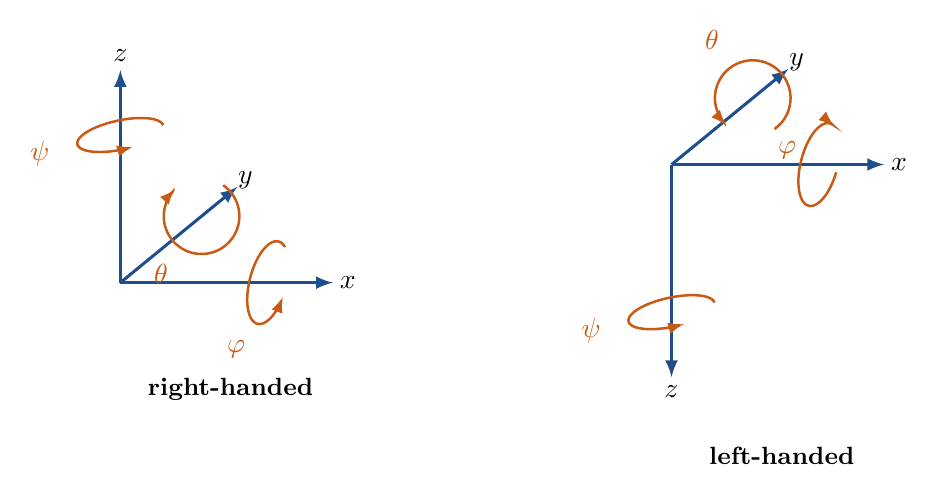
\begin{tikzpicture}
    \coordframe{(1cm,0cm)}{(0.55cm,0.45cm)}{(0cm,1cm)}{right-handed}{$\varphi$}{$\theta$}{$\psi$}{-1.35}
    \begin{scope}[xshift=7cm, yshift=1.5cm]
      \coordframe{(1cm,0cm)}{(0.55cm,0.45cm)}{(0cm,-1cm)}{left-handed}{$\varphi$}{$\theta$}{$\psi$}{-3.7}
    \end{scope}
  \end{tikzpicture}
  \caption{Example~1: the left-handed system differs from the right-handed system only by the
  opposite $z$ axis.}
  \label{fig:ex1}
\end{figure}

The left-handed system in Figure~\ref{fig:ex1} equals the right-handed system except for the
opposite $z$ axis, i.e.\ $\vect P = \vect S = \operatorname{diag}(1,1,-1)$. Let the pose
$\vect T_r = \begin{bmatrix} \vect R_r & \vect t_r \\ \vect 0^T & 1 \end{bmatrix}$ with
$\vect t_r = (x, y, z)^T$ be given. We look for the pose $(q_l, \vect t_l)$ in the left-handed
system.

\paragraph{Position.} $\vect t_l = \vect S \vect t_r = (x,\, y,\, -z)^T$.

\paragraph{Rotation matrices.} With the YXZ convention \eqref{eq:yxz},
\begin{equation}
  \vect R_r = \vect R_y(\theta)\vect R_x(\varphi)\vect R_z(\psi) =
  \begin{bmatrix}
    c_3c_2 + s_1s_3s_2 & c_3s_1s_2 - c_2s_3 & c_1s_2 \\
    c_1s_3 & c_1c_3 & -s_1 \\
    c_2s_1s_3 - c_3s_2 & s_3s_2 + c_3c_2s_1 & c_1c_2
  \end{bmatrix}.
\end{equation}
In the left-handed system the angles $(\varphi, \theta, \psi)$ become $(-\varphi, -\theta, \psi)$
by Remark~\ref{rem:angles}, and
\begin{equation}
  \vect R_l = \vect R_y(-\theta)\vect R_x(-\varphi)\vect R_z(\psi) = \vect S \vect R_r \vect S =
  \begin{bmatrix}
    c_3c_2 + s_1s_3s_2 & c_3s_1s_2 - c_2s_3 & -c_1s_2 \\
    c_1s_3 & c_1c_3 & s_1 \\
    c_3s_2 - c_2s_1s_3 & -s_3s_2 - c_3c_2s_1 & c_1c_2
  \end{bmatrix}.
\end{equation}

\paragraph{Quaternions via rotation matrices.} By \eqref{eq:rotm2quat}, with
\begin{equation}
  q_s = \frac{\sqrt{c_1c_3 + c_1c_2 + c_3c_2 + s_1s_3s_2 + 1}}{2},
\end{equation}
the right-handed (left column) and the left-handed system (right column) give
\begin{align}
  q_{s,r} &= q_s, & q_{s,l} &= q_s, \\
  q_{x,r} &= \frac{s_1 + s_3s_2 + c_3c_2s_1}{4q_s}, & q_{x,l} &= -\frac{s_1 + s_3s_2 + c_3c_2s_1}{4q_s}, \\
  q_{y,r} &= \frac{c_1s_2 + c_3s_2 - c_2s_1s_3}{4q_s}, & q_{y,l} &= -\frac{c_1s_2 + c_3s_2 - c_2s_1s_3}{4q_s}, \\
  q_{z,r} &= \frac{c_1s_3 + c_2s_3 - c_3s_1s_2}{4q_s}, & q_{z,l} &= \phantom{-}\frac{c_1s_3 + c_2s_3 - c_3s_1s_2}{4q_s}.
\end{align}

\paragraph{Quaternions from Euler angles.} Directly,
\begin{align}
  q_{r,\mathrm{eul}} = q_y(\theta)\,q_x(\varphi)\,q_z(\psi) = \bigl(
    &s_{1h}s_{3h}s_{2h} + c_{1h}c_{3h}c_{2h},\;
     c_{3h}c_{2h}s_{1h} + c_{1h}s_{3h}s_{2h}, \nonumber\\
    &c_{1h}c_{3h}s_{2h} - c_{2h}s_{1h}s_{3h},\;
     c_{1h}c_{2h}s_{3h} - c_{3h}s_{1h}s_{2h} \bigr), \\
  q_{l,\mathrm{eul}} = q_y(-\theta)\,q_x(-\varphi)\,q_z(\psi) = \bigl(
    &s_{1h}s_{3h}s_{2h} + c_{1h}c_{3h}c_{2h},\;
     -c_{3h}c_{2h}s_{1h} - c_{1h}s_{3h}s_{2h}, \nonumber\\
    &c_{2h}s_{1h}s_{3h} - c_{1h}c_{3h}s_{2h},\;
     c_{1h}c_{2h}s_{3h} - c_{3h}s_{1h}s_{2h} \bigr).
\end{align}

\paragraph{Both ways agree.}
Since $\vect R_r = \vect R(q_{r,\mathrm{eul}})$, \eqref{eq:rotm2quat} gives
$q_{r,\mathrm{rotm}} = q_{r,\mathrm{eul}}$ in all four components provided
$q_{s,\mathrm{eul}} > 0$, and likewise in the left-handed system. For the scalar part this can be
checked directly with $\sin(2x) = 2\sin x\cos x$, $\sin^2 x = \frac12(1-\cos 2x)$ and
$\cos^2 x = \frac12(1+\cos 2x)$:
\begin{align}
  q_{s,\mathrm{eul}}^2
  &= \bigl(s_{1h}s_{2h}s_{3h} + c_{1h}c_{2h}c_{3h}\bigr)^2
   = s_{1h}^2s_{2h}^2s_{3h}^2 + c_{1h}^2c_{2h}^2c_{3h}^2
     + 2\, s_{1h}c_{1h}\, s_{2h}c_{2h}\, s_{3h}c_{3h} \nonumber\\
  &= \tfrac18 (1-c_1)(1-c_2)(1-c_3) + \tfrac18 (1+c_1)(1+c_2)(1+c_3) + \tfrac14 s_1s_2s_3 \nonumber\\
  &= \tfrac18 \bigl(2 + 2c_1c_2 + 2c_1c_3 + 2c_2c_3\bigr) + \tfrac14 s_1s_2s_3
   = \frac{1 + c_1c_2 + c_1c_3 + c_2c_3 + s_1s_2s_3}{4}
   = q_{s,\mathrm{rotm}}^2 .
\end{align}
With $q_{s,\mathrm{eul}} > 0$ it follows that $q_{s,\mathrm{eul}} = q_{s,\mathrm{rotm}}$.

For the vector part it suffices to show $4\,q_{s,\mathrm{eul}}\,q_{x,\mathrm{eul}} = R_{32} - R_{23}$
etc., since dividing by $4q_s$ then gives \eqref{eq:rotm2quat}. Besides the identities above,
$4\,s_{kh}c_{kh}\,s_{mh}c_{mh} = s_k s_m$, $s_{kh}^2 + c_{kh}^2 = 1$, $s_{kh}^2 - c_{kh}^2 = -c_k$,
and
\begin{equation}
  s_{kh}^2 s_{mh}^2 + c_{kh}^2 c_{mh}^2 = \tfrac12 (1 + c_k c_m), \qquad
  c_{kh}^2 c_{mh}^2 - s_{kh}^2 s_{mh}^2 = \tfrac12 (c_k + c_m)
\end{equation}
are used. Grouping the products by the angle that appears squared gives
\begin{align}
  4\,q_{s,\mathrm{eul}}\,q_{x,\mathrm{eul}}
  &= 4\bigl(s_{1h}s_{2h}s_{3h} + c_{1h}c_{2h}c_{3h}\bigr)\bigl(c_{2h}c_{3h}s_{1h} + c_{1h}s_{2h}s_{3h}\bigr) \nonumber\\
  &= 4\, s_{2h}c_{2h}\, s_{3h}c_{3h} \bigl(s_{1h}^2 + c_{1h}^2\bigr)
   + 4\, s_{1h}c_{1h} \bigl(s_{2h}^2 s_{3h}^2 + c_{2h}^2 c_{3h}^2\bigr) \nonumber\\
  &= s_2 s_3 + s_1 (1 + c_2 c_3)
   = s_1 + s_3s_2 + c_3c_2s_1 = R_{32} - R_{23}, \\[4pt]
  4\,q_{s,\mathrm{eul}}\,q_{y,\mathrm{eul}}
  &= 4\bigl(s_{1h}s_{2h}s_{3h} + c_{1h}c_{2h}c_{3h}\bigr)\bigl(c_{1h}c_{3h}s_{2h} - c_{2h}s_{1h}s_{3h}\bigr) \nonumber\\
  &= 4\, s_{1h}c_{1h}\, s_{3h}c_{3h} \bigl(s_{2h}^2 - c_{2h}^2\bigr)
   + 4\, s_{2h}c_{2h} \bigl(c_{1h}^2 c_{3h}^2 - s_{1h}^2 s_{3h}^2\bigr) \nonumber\\
  &= -s_1 s_3 c_2 + s_2 (c_1 + c_3)
   = c_1s_2 + c_3s_2 - c_2s_1s_3 = R_{13} - R_{31}, \\[4pt]
  4\,q_{s,\mathrm{eul}}\,q_{z,\mathrm{eul}}
  &= 4\bigl(s_{1h}s_{2h}s_{3h} + c_{1h}c_{2h}c_{3h}\bigr)\bigl(c_{1h}c_{2h}s_{3h} - c_{3h}s_{1h}s_{2h}\bigr) \nonumber\\
  &= 4\, s_{1h}c_{1h}\, s_{2h}c_{2h} \bigl(s_{3h}^2 - c_{3h}^2\bigr)
   + 4\, s_{3h}c_{3h} \bigl(c_{1h}^2 c_{2h}^2 - s_{1h}^2 s_{2h}^2\bigr) \nonumber\\
  &= -s_1 s_2 c_3 + s_3 (c_1 + c_2)
   = c_1s_3 + c_2s_3 - c_3s_1s_2 = R_{21} - R_{12}.
\end{align}
Hence $q_{r,\mathrm{rotm}} = q_{r,\mathrm{eul}}$ in all four components. In the left-handed system,
$\vect R_l = \vect S\vect R_r\vect S$ leaves the trace unchanged and flips the sign of
$R_{32} - R_{23}$ and $R_{13} - R_{31}$, while $q_{l,\mathrm{eul}}$ differs from $q_{r,\mathrm{eul}}$
by the same signs. So $q_{l,\mathrm{rotm}} = q_{l,\mathrm{eul}}$ as well. All four components are
also proved in Lean (Section~\ref{sec:lean}).

\paragraph{Result.} By Theorem~\ref{thm:main} with $-\vect S\vect v = (-q_x, -q_y, q_z)^T$:
\begin{equation}\label{eq:rule1}
  \begin{pmatrix} q_s \\ q_x \\ q_y \\ q_z \end{pmatrix}_{\!\text{right}}
  \longleftrightarrow
  \begin{pmatrix} q_s \\ -q_x \\ -q_y \\ q_z \end{pmatrix}_{\!\text{left}},
  \qquad
  \begin{pmatrix} x \\ y \\ z \end{pmatrix}_{\!\text{right}}
  \longleftrightarrow
  \begin{pmatrix} x \\ y \\ -z \end{pmatrix}_{\!\text{left}}.
\end{equation}

%======================================================================
\section{Example 2: swapped \texorpdfstring{$y$}{y} and \texorpdfstring{$z$}{z} axes (Unity3D)}\label{sec:ex2}

\begin{figure}[H]
  \centering
  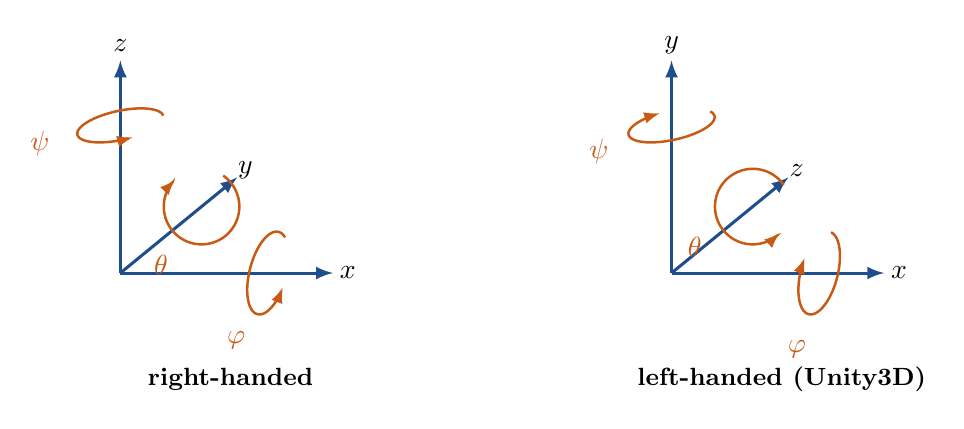
\begin{tikzpicture}
    \coordframe{(1cm,0cm)}{(0.55cm,0.45cm)}{(0cm,1cm)}{right-handed}{$\varphi$}{$\theta$}{$\psi$}{-1.35}
    \begin{scope}[xshift=7cm]
      \coordframe{(1cm,0cm)}{(0cm,1cm)}{(0.55cm,0.45cm)}{left-handed (Unity3D)}{$\varphi$}{$\psi$}{$\theta$}{-1.35}
    \end{scope}
  \end{tikzpicture}
  \caption{Example~2: the left-handed system of Unity3D results from the right-handed system by
  swapping the $y$ and $z$ axes. Each angle belongs to the same physical axis in both systems.}
  \label{fig:ex2}
\end{figure}

In Unity3D (Figure~\ref{fig:ex2}) the $y$ and $z$ axes are swapped with respect to the
right-handed system:
\begin{equation}
  \vect P = \begin{bmatrix} 1 & 0 & 0 \\ 0 & 0 & 1 \\ 0 & 1 & 0 \end{bmatrix},\qquad
  \vect t_l = \vect P \vect t_r = (x,\, z,\, y)^T .
\end{equation}
Unity uses the order YXZ in its own system. In the right-handed system this corresponds to
$\vect R_z \vect R_x \vect R_y$:
\begin{equation}
  \vect R_r = \vect R_z(\psi)\vect R_x(\varphi)\vect R_y(\theta) =
  \begin{bmatrix}
    c_3c_2 - s_3s_2s_1 & -c_1s_3 & c_3s_2 + c_2s_3s_1 \\
    c_2s_3 + c_3s_2s_1 & c_3c_1 & s_3s_2 - c_3c_2s_1 \\
    -c_1s_2 & s_1 & c_2c_1
  \end{bmatrix}.
\end{equation}
With $\vect P \vect R_z(\psi) \vect P = \vect R_y(-\psi)$, $\vect P \vect R_x(\varphi) \vect P = \vect R_x(-\varphi)$
and $\vect P \vect R_y(\theta) \vect P = \vect R_z(-\theta)$,
\begin{equation}
  \vect R_l = \vect R_y(-\psi)\vect R_x(-\varphi)\vect R_z(-\theta) = \vect P \vect R_r \vect P =
  \begin{bmatrix}
    c_3c_2 - s_3s_2s_1 & c_3s_2 + c_2s_3s_1 & -c_1s_3 \\
    -c_1s_2 & c_2c_1 & s_1 \\
    c_2s_3 + c_3s_2s_1 & s_3s_2 - c_3c_2s_1 & c_3c_1
  \end{bmatrix}.
\end{equation}
The quaternions from the Euler angles are
\begin{align}
  q_r = q_z(\psi)\,q_x(\varphi)\,q_y(\theta) = \bigl(
    &c_{3h}c_{2h}c_{1h} - s_{3h}s_{2h}s_{1h},\;
     c_{3h}c_{2h}s_{1h} - c_{1h}s_{3h}s_{2h}, \nonumber\\
    &c_{3h}c_{1h}s_{2h} + c_{2h}s_{3h}s_{1h},\;
     c_{2h}c_{1h}s_{3h} + c_{3h}s_{2h}s_{1h} \bigr), \\
  q_l = q_y(-\psi)\,q_x(-\varphi)\,q_z(-\theta) = \bigl(
    &c_{3h}c_{2h}c_{1h} - s_{3h}s_{2h}s_{1h},\;
     c_{1h}s_{3h}s_{2h} - c_{3h}c_{2h}s_{1h}, \nonumber\\
    &-c_{2h}c_{1h}s_{3h} - c_{3h}s_{2h}s_{1h},\;
     -c_{3h}c_{1h}s_{2h} - c_{2h}s_{3h}s_{1h} \bigr).
\end{align}
The conversion via \eqref{eq:rotm2quat} yields the same quaternions for $q_s > 0$.

\paragraph{Result.} With $-\vect P\vect v = (-q_x, -q_z, -q_y)^T$:
\begin{equation}\label{eq:rule2}
  \begin{pmatrix} q_s \\ q_x \\ q_y \\ q_z \end{pmatrix}_{\!\text{right}}
  \longleftrightarrow
  \begin{pmatrix} q_s \\ -q_x \\ -q_z \\ -q_y \end{pmatrix}_{\!\text{left}},
  \qquad
  \begin{pmatrix} x \\ y \\ z \end{pmatrix}_{\!\text{right}}
  \longleftrightarrow
  \begin{pmatrix} x \\ z \\ y \end{pmatrix}_{\!\text{left}}.
\end{equation}

%======================================================================
\section{Common pitfalls}\label{sec:pitfalls}

\begin{enumerate}
  \item \textbf{Permuting without sign change.} Mapping the vector part like a position,
        $q_l = (q_s, \vect P\vect v)$, gives the conjugate of the correct quaternion, i.e.\ the
        inverse rotation. Small rotations then look plausible but turn the wrong way. The correct
        rule is $q_l = (q_s, -\vect P\vect v)$.
  \item \textbf{Component order.} Libraries store quaternions as $(q_s, q_x, q_y, q_z)$ or as
        $(q_x, q_y, q_z, q_s)$. Unity and ROS messages use the latter, Eigen's constructor takes the
        scalar part first. The rules in this paper refer to the components, not to array positions.
  \item \textbf{Quaternion algebra convention.} Quaternions in the JPL convention ($ij = -k$) are
        the conjugates of Hamilton quaternions \cite{sola2017, sommer2018}. Mixing both conventions
        also flips the sign of the vector part, but this is not a change of handedness.
  \item \textbf{Euler angles.} The angle values cannot be reused in the new system with the same
        axis sequence. Each elementary rotation is mapped to the corresponding axis of the new
        system, and its angle changes sign unless the axis itself is mirrored
        (Remark~\ref{rem:angles}). In Example~2 the right-handed sequence $z$, $x$, $y$ becomes
        Unity's $y$, $x$, $z$.
  \item \textbf{Intrinsic vs.\ extrinsic.} The same three angles describe different rotations
        depending on whether they refer to moving or fixed axes. The conversion must keep the
        interpretation.
  \item \textbf{Active vs.\ passive.} Whether $\vect R$ maps local to global coordinates or the
        other way round does not affect the rule, since $(\vect P \vect R \vect P^T)^T =
        \vect P \vect R^T \vect P^T$ and the rule commutes with conjugation. It must, however, be
        the same on both sides.
  \item \textbf{Sign ambiguity.} $q$ and $-q$ are the same rotation. Comparing converted quaternions
        component by component can therefore fail although the rotations agree.
  \item \textbf{Changing coordinates vs.\ mirroring the object.} The rule describes the same physical
        pose in another coordinate system. Mirroring an object inside one system is a different
        operation and changes its geometry.
\end{enumerate}

%======================================================================
\section{Formal verification in Lean 4}\label{sec:lean}

All statements about both examples were proved formally in the proof assistant Lean~4
\cite{lean4} with the library Mathlib \cite{mathlib} (both version~4.15.0). The source code is in
the folder \texttt{lean/} of the project. The proofs contain no \lean{sorry} and are checked with
\begin{center}
  \texttt{lake exe cache get \&\& lake build}
\end{center}
The quaternions are those of Mathlib (\texttt{Quaternion}~$\R$) with the Hamilton product, and
\lean{rotm2quat} is formula~\eqref{eq:rotm2quat}. Every statement about rotm2quat assumes
$q_s > 0$.

{\sloppy The proof follows the structure of Section~\ref{sec:prelim}: $\vect R(q)$ is multiplicative
(\lean{rotmOf\_mul}), the elementary rotations are $\vect R(q_x)$, $\vect R(q_y)$, $\vect R(q_z)$
(\lean{Rx\_eq} etc.), and rotm2quat inverts $\vect R(\cdot)$ on unit quaternions with $q_s > 0$
(\lean{rotm2quat\_rotmOf}). Reflection and axis swap commute with $\vect R(\cdot)$
(\lean{S\_rotmOf\_S}, \lean{P2\_rotmOf\_P2}).\par}

\begin{table}[H]
  \centering
  \footnotesize
  \begin{tabular}{@{}lll@{}}
    \toprule
    Statement & Example 1 & Example 2 \\
    \midrule
    Rotation matrices $\vect R_r$, $\vect R_l$ explicit & \lean{Rr\_explicit}, \lean{Rl\_explicit} & \lean{R2r\_explicit}, \lean{R2l\_explicit} \\
    $\vect R_l = \vect P \vect R_r \vect P$ & \lean{Rl\_eq\_S\_Rr\_S} & \lean{R2l\_eq\_P2\_R2r\_P2} \\
    eul2quat explicit & \lean{qr\_explicit}, \lean{ql\_explicit} & \lean{q2r\_explicit}, \lean{q2l\_explicit} \\
    rotm2quat explicit & \lean{rotm2quat\_Rr\_explicit}, \lean{\dots Rl\dots} & -- \\
    rotm2quat $=$ eul2quat (all 4 comp.) & \lean{eul\_eq\_rotm\_right}, \lean{\dots left} & \lean{rotm2quat\_R2r}, \lean{rotm2quat\_R2l} \\
    Rule right $\to$ left & \lean{rotm2quat\_left\_eq\_toLeft} & \lean{rotm2quat\_left2\_eq\_toLeft2} \\
    Rule left $\to$ right & \lean{rotm2quat\_right\_eq\_toLeft} & \lean{rotm2quat\_right2\_eq\_toLeft2} \\
    Position & \lean{position\_left} & \lean{position\_left2} \\
    \bottomrule
  \end{tabular}
  \caption{Lean theorems for the statements of this paper}
  \label{tab:lean}
\end{table}

Theorem~\ref{thm:main} for arbitrary $\vect P$ is not formalized, only its two special cases.

%======================================================================
\section{Conclusion}\label{sec:conclusion}

The conversion between right-handed and left-handed systems is widely used but rarely derived.
If a right-handed and a left-handed system differ by an orthogonal matrix $\vect P$ with
$\det \vect P = -1$, the position is transformed with $\vect P$ and the vector part of the
quaternion with $-\vect P$, while the scalar part stays the same. For a mirrored $z$ axis this
gives $(q_s, -q_x, -q_y, q_z)$, for Unity3D $(q_s, -q_x, -q_z, -q_y)$. In both cases the rule is its
own inverse. Both cases are proved formally in Lean~4, including the agreement of the conversion via
rotation matrices with the direct conversion from Euler angles in all four quaternion components.

\bibliographystyle{IEEEtran}
\bibliography{IEEEabrv,bibliography}

\end{document}
